\documentclass[14pt]{beamer}
\usepackage{./Estilos/BeamerUVM}
\usepackage{./Estilos/ColoresLatex}
\usepackage{circuitikz}
\usepackage{schemata}
\usetheme{Warsaw}
\usecolortheme{rose}
%\useoutertheme{default}
\setbeamercovered{invisible}
% or whatever (possibly just delete it)
\setbeamertemplate{section in toc}[sections numbered]
\setbeamertemplate{subsection in toc}[subsections numbered]
\setbeamertemplate{subsection in toc}{\leavevmode\leftskip=3.2em\rlap{\hskip-2em\inserttocsectionnumber.\inserttocsubsectionnumber}\inserttocsubsection\par}
%\setbeamercolor{section in toc}{fg=blue}
%\setbeamercolor{subsection in toc}{fg=blue}
%\setbeamercolor{frametitle}{fg=blue}
\setbeamertemplate{caption}[numbered]

\setbeamertemplate{footline}
\beamertemplatenavigationsymbolsempty
\setbeamertemplate{headline}{}


\makeatletter
\setbeamercolor{section in foot}{bg=gray!30, fg=black!90!orange}
\setbeamercolor{subsection in foot}{bg=blue!30}
\setbeamercolor{date in foot}{bg=black}
\setbeamertemplate{footline}
{
  \leavevmode%
  \hbox{%
  \begin{beamercolorbox}[wd=.333333\paperwidth,ht=2.25ex,dp=1ex,center]{section in foot}%
    \usebeamerfont{section in foot} \insertsection
  \end{beamercolorbox}%
  \begin{beamercolorbox}[wd=.333333\paperwidth,ht=2.25ex,dp=1ex,center]{subsection in foot}%
    \usebeamerfont{subsection in foot}  \insertsubsection
  \end{beamercolorbox}%
  \begin{beamercolorbox}[wd=.333333\paperwidth,ht=2.25ex,dp=1ex,right]{date in head/foot}%
    \usebeamerfont{date in head/foot} \hspace*{2em}
    \insertframenumber{} / \inserttotalframenumber \hspace*{2ex} 
  \end{beamercolorbox}}%
  \vskip0pt%
}
\makeatother

\makeatletter
\patchcmd{\beamer@sectionintoc}{\vskip1.5em}{\vskip0.8em}{}{}
\makeatother
% \usefonttheme{serif}
\usepackage[clock]{ifsym}
\DeclareSIUnit\erg{erg}
\DeclareSIUnit[number-unit-product = {\,}]\cal{cal}

\sisetup{per-mode=symbol}
\resetcounteronoverlays{saveenumi}

% Macro para agregar el logo de UVM en cada slide de la presentación

\addtobeamertemplate{frametitle}{}{%
\begin{tikzpicture}[remember picture,overlay]
\coordinate (logo) at ([xshift=-1.5cm,yshift=-0.8cm]current page.north east);
% \fill[devryblue] (logo) circle (.9cm);
% \clip (logo) circle (.75cm);
\node at (logo) {
\includegraphics[width=2.1cm]{Imagenes/logo_UVM.png}};
\end{tikzpicture}}


\title{\Large{Potencial de acción} \\ \normalsize{Física IV (Área II)}}
\date{}

\begin{document}
\maketitle

\section*{Contenido}
\frame[allowframebreaks]{\frametitle{Contenido} \tableofcontents[currentsection, hideallsubsections]}


\section{El potencial de equilibrio}
\frame{\tableofcontents[currentsection, hideothersubsections]}
\subsection{}

\begin{frame}
\frametitle{¿Qué es el potencial de equilibrio?}
Toda célula está delimitada por una membrana plasmática formada por una bicapa de lípidos, lo que le confiere un carácter \textocolor{byzantine}{hidrofóbico}.
\end{frame}
\begin{frame}
\frametitle{Permeabilidad de la membrana}
No obstante, la membrana es semipermeable a una amplia variedad de moléculas, \pause lo que resulta en una diferencia en la composición del citoplasma y el medio extracelular.
\end{frame}
\begin{frame}
\frametitle{Permeabilidad de la membrana}
De entre todas las moléculas, \pause los iones resultan ser de vital importancia para múltiples funciones celulares.
\end{frame}
\begin{frame}
\frametitle{¿Qué es un ion?}
Un ion es un átomo o molécula que \textocolor{burgundy}{ha ganado} o \textocolor{carmine}{perdido} uno o más electrones, lo que resulta en una carga eléctrica neta.
\end{frame}
\begin{frame}
\frametitle{¿Qué es un ion?}
Esta carga eléctrica puede ser positiva si el ion ha \textocolor{cerulean}{perdido electrones} (llamado \textocolor{cerulean}{catión}) \pause o negativa si ha \textocolor{coralred}{ganado electrones} (llamado \textocolor{coralred}{anión}).
\end{frame}
\begin{frame}
\frametitle{Permeabilidad de la membrana}
Los más abundantes son el Na+, K+, Ca2+ y Cl-, cuyos valores fisiológicos en el humano se indican en la siguiente tabla.
\end{frame}
\begin{frame}
\frametitle{Iones en el cuerpo humano}
\vspace*{-0.5cm}
\begin{table}
    \centering
    \begin{tabular}{l | c | c}
    Ion & C. intracelular & C. extracelular \\ \hline
    Na+ & 12 mM & 145 mM \\ \hline
    K+ & 155 mM & 4 mM \\ \hline
    Ca++ & 100 mM & 1.5 mM \\ \hline
    Cl- & 4.2 mM & 123 mM \\ \hline
\end{tabular}
\end{table}
\end{frame}
\begin{frame}
\frametitle{Unidades de la tabla}
Recordemos que: \textbf{mM}: \pause Milimolar, es una medida de concentración de un soluto en una disolución (\num{d-3} molar).
\end{frame}
\begin{frame}
\frametitle{Diferencia de concentraciones}
Esta diferencia en las concentraciones iónicas condiciona una \textocolor{debianred}{diferencia entre las cargas} a ambos lados de la membrana, \pause las mismas que tratarán de igualarse (\textocolor{cobalt}{equilibrio de Gibbs-Donnan}).
\end{frame}
\begin{frame}
\frametitle{Paso de iones}
Bajo ciertas condiciones, la membrana permite el paso de algunos iones, \pause lo que genera un \textocolor{red}{flujo de cargas} que depende de la permeabilidad relativa de la membrana a cada ion.
\end{frame}
\begin{frame}
\frametitle{Potencial de membrana}
Al pasar los iones a favor de su \textocolor{armygreen}{gradiente de concentración} (de donde hay más a donde hay menos) \pause se genera una \textocolor{byzantium}{diferencia de potencial eléctrico} a través de la membrana, \pause llamado \textocolor{red}{potencial de membrana} (medida en milivoltios o mV).
\end{frame}
\begin{frame}
\frametitle{Potecial de membrana}
Es de crucial importancia comprender que dicho potencial de membrana será determinado solo por las \textocolor{auburn}{concentraciones iónicas} a cada lado de la membrana \pause y por la \textocolor{bondiblue}{permeabilidad} de la misma membrana a cada ion.
\end{frame}
\begin{frame}
\frametitle{Potencial de inicio}
\vspace*{-0.75cm}
\begin{figure}
    \centering
    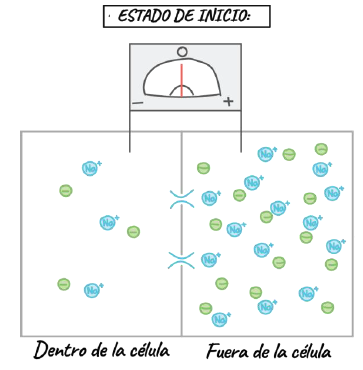
\includegraphics[scale=0.6]{Imagenes/Potencial_Accion_04.png}
\end{figure}
\end{frame}
\begin{frame}
\frametitle{Estado de inicio}
En el estadio inicial, tenemos dos compartimentos, \textocolor{ao}{adentro} y \textocolor{red}{afuera} de la célula, \pause y podemos ver que afuera de la célula hay mucho Na+ y Cl-.
\end{frame}
\begin{frame}
\frametitle{Estado de inicio}
En este caso, la membrana es \textocolor{bulgarianrose}{IMPERMEABLE} al Cl- \pause pero \textocolor{cadmiumgreen}{PERMEABLE} al Na+, \pause porque existen canales de Na que permitirán que éste difunda hacia adentro de la célula (a favor del gradiente de concentración)
\end{frame}
\begin{frame}
\frametitle{Potencial de equilibrio}
Y así el Na+,  \textocolor{cadet}{comenzará a difundir} hacia adentro de la célula.
\end{frame}
\begin{frame}
\frametitle{Potencial de equilibrio}
Pero llegará el momento en donde se \textocolor{carnelian}{detendrá su difusión} \pause porque las cargas del Cl- se encuentran atrayendo al Na+ para que regrese al medio extracelular, \pause en este momento el Na+ ha llegado a su \textocolor{ceruleanblue}{POTENCIAL DE EQUILIBRIO}.
\end{frame}
\begin{frame}
\frametitle{Potencial de equilibrio}
\vspace*{-0.75cm}
\begin{figure}
    \centering
    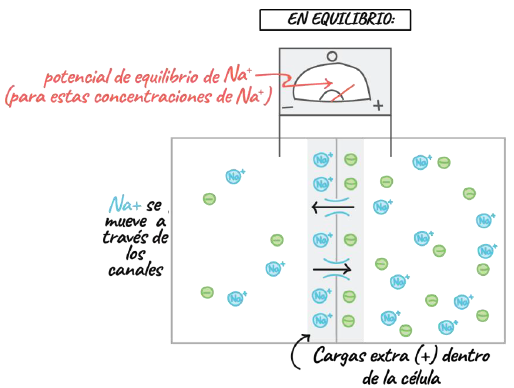
\includegraphics[scale=0.6]{Imagenes/Potencial_Accion_05.png}
\end{figure}
\end{frame}
\begin{frame}
\frametitle{Ecuación de Nerst}
Este equilibrio está descrito por la \textocolor{cinnabar}{ecuación de Nernst}, y se aplica para cada ion difusible a través de la membrana celular:
\end{frame}
\begin{frame}
\frametitle{Ecuación de Nerst}
\vspace*{-1cm}
\begin{align*}
E_{i} = \dfrac{R \, T}{z \, F} \, \ln \dfrac{\left[ \text{ion} \right]_{e}}{\left[ \text{ion} \right]_{i}}
\end{align*}
donde:
\setbeamercolor{item projected}{bg=bananayellow,fg=black}
\setbeamertemplate{enumerate items}{%
\usebeamercolor[bg]{item projected}%
\raisebox{1.5pt}{\colorbox{bg}{\color{fg}\footnotesize\insertenumlabel}}%
}
\begin{enumerate}[<+->]
\item $E_{i}$ es el potencial de equilibrio del ion X [V]
\item $R$ constante de los gases (\num{8.315} \unit{\joule\per{\kelvin\mol}})
\item $T$ temperatura en grados Kelvin
\seti
\end{enumerate}
\end{frame}
\begin{frame}
\frametitle{Ecuación de Nerst}
\vspace*{-1cm}
\begin{align*}
E_{i} = \dfrac{R \, T}{z \, F} \, \ln \dfrac{\left[ \text{ion} \right]_{e}}{\left[ \text{ion} \right]_{i}}
\end{align*}
\setbeamercolor{item projected}{bg=bananayellow,fg=black}
\setbeamertemplate{enumerate items}{%
\usebeamercolor[bg]{item projected}%
\raisebox{1.5pt}{\colorbox{bg}{\color{fg}\footnotesize\insertenumlabel}}%
}
\begin{enumerate}[<+->]
\conti
\item $z$ valencia del ion $(-1)$ para aniones y $(+1)$ para cationes monovalentes.
\item $F$ = constante de Faraday (\SI{9.648d4}{\coulomb\per\mol})
\seti
\end{enumerate}
\end{frame}
\begin{frame}
\frametitle{Ecuación de Nerst}
\vspace*{-1cm}
\begin{align*}
E_{i} = \dfrac{R \, T}{z \, F} \, \ln \dfrac{\left[ \text{ion} \right]_{e}}{\left[ \text{ion} \right]_{i}}
\end{align*}
\setbeamercolor{item projected}{bg=bananayellow,fg=black}
\setbeamertemplate{enumerate items}{%
\usebeamercolor[bg]{item projected}%
\raisebox{1.5pt}{\colorbox{bg}{\color{fg}\footnotesize\insertenumlabel}}%
}
\begin{enumerate}[<+->]
\conti
\item $\left[ \text{ion} \right]_{e}$ es la concentración extracelular del ion.
\item $\left[ \text{ion} \right]_{i}$ es la concentración intracelular del ion.
\end{enumerate}
\end{frame}

\subsection{Potencial de membrana en reposo}

\begin{frame}
\frametitle{Permeabilidad de la membrana}
Considerando que la membrana plasmática \textocolor{debianred}{es principalmente permeable} al K+, \pause debido a la presencia de canales de fuga de K+ que permiten que éste salga de la célula cuando se encuentra en reposo.
\end{frame}
\begin{frame}
\frametitle{Permeabilidad de la membrana}
Se puede simplificar el potencial de membrana en reposo como el potencial de equilibrio de K+.
\end{frame}
\begin{frame}
\frametitle{Permeabilidad de la membrana}
Usando la ecuación de Nernst, usando los valores conocidos, tenemos:
\end{frame}
\begin{frame}
\frametitle{Permeabilidad de la membrana}
\begin{eqnarray*}
\begin{aligned}
E_{K+} &= \dfrac{\left( \SI{8.315}{\joule\per{\kelvin\mol}} \right) \left( \SI{310.16}{\kelvin} \right) }{(+1)\left( \SI{9.648d4}{\coulomb\per\mol} \right)} {\times} \, \ln   \left( \dfrac{\left[ 4 \, \text{mM} \right]}{\left[ 155 \, \text{mM} \right]} \right) \\ \pause
E_{K+} &= \left( \SI{0.2673}{\joule\coulomb} \right) \left( -3.6571 \right) \\ \pause
E_{K+} &= -\SI{0.09776}{\volt} = \pause -\SI{97.8}{\milli\volt}
\end{aligned}
\end{eqnarray*}
\end{frame}
\begin{frame}
\frametitle{Valor cercano al potencial reposo}
El potencial de equilibrio para el K+ es $-\SI{97.8}{\milli\volt}$ \pause y a este voltaje se acercará el potencial de membrana en reposo.
\end{frame}
\begin{frame}
\frametitle{Potencial reposo}
Sin embargo, el potencial de membrana en reposo de las células es diferente, ya que también las células también son permeable as a otros iones como el Na+ y Cl-.
\end{frame}

\section{Potencial de acción}
\frame{\tableofcontents[currentsection, hideothersubsections]}
\subsection{Definición}

\begin{frame}
\frametitle{El potencial de acción}
Algunos tipos de células tienen la capacidad de cambiar el potencial de membrana en reposo que es negativo, \pause y generar \textocolor{ao}{potenciales positivos} y transientes \pause que conocemos como \textocolor{red}{potenciales de acción.}
\end{frame}
\begin{frame}
\frametitle{El potencial de acción}
Los potenciales de acción son cambios estereotípicos, abruptos y transitorios en el potencial de membrana que ocurren en células excitables.
\end{frame}
\begin{frame}
\frametitle{Célula excitable}
Se llaman así porque pueden responder ante la estimulación directa con una corriente eléctrica (por ejemplo, neuronas, células musculares y células endocrinas).
\end{frame}
\begin{frame}
\frametitle{El potencial de acción}
Los potenciales de acción desempeñan un papel central en la comunicación de celular.
\end{frame}
\begin{frame}
\frametitle{El potencial de acción}
Siendo la base de la propagación de señales en neuronas \pause y activando diversos procesos intracelulares como la contracción muscular y la liberación de insulina en las células beta del páncreas.
\end{frame}

\subsection{Fundamentos del potencial de acción}

\begin{frame}
\frametitle{¿Cómo se presenta?}
El potencial de acción se debe a que existe un \textocolor{byzantine}{estímulo específico} \pause que abre canales de Na+ dependientes de voltaje.
\end{frame}
\begin{frame}
\frametitle{¿Cómo se presenta?}
Hasta que son tantos que el Na+ comienza a difundir desde afuera de la célula al interior, haciendo el citosol más positivo.
\end{frame}
\begin{frame}
\frametitle{¿Cómo se presenta?}
Es por ello por lo que el potencial de acción se acerca al potencial de equilibrio del Na+, \pause porque con la apertura de estos canales, se aumenta su permeabilidad y el Na+ busca llegar a su equilibrio.
\end{frame}

\subsection{Fases del potencial de acción}

\begin{frame}
\frametitle{Fases del potencial}
El potencial de acción pasa por distintas fases dependiendo del tipo de célula excitable.
\end{frame}
\begin{frame}
\frametitle{El estímulo}
Para iniciar el potencial de acción, se tiene que generar un estímulo que alcance el \textocolor{coquelicot}{umbral}.
\end{frame}
\begin{frame}
\frametitle{El estímulo}
\begin{figure}
    \centering
    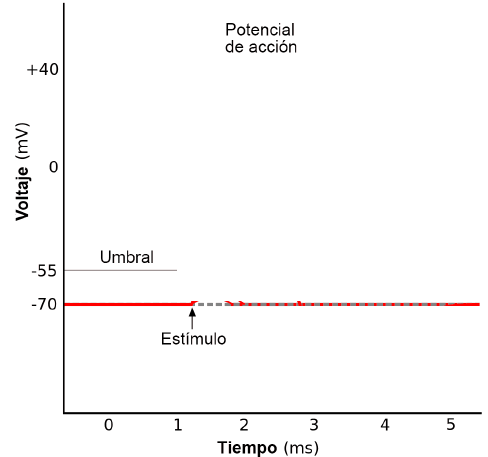
\includegraphics[scale=0.5]{Imagenes/Potencial_Accion_08a.png}
\end{figure}
\end{frame}
\begin{frame}
\frametitle{El estímulo}
\begin{figure}
    \centering
    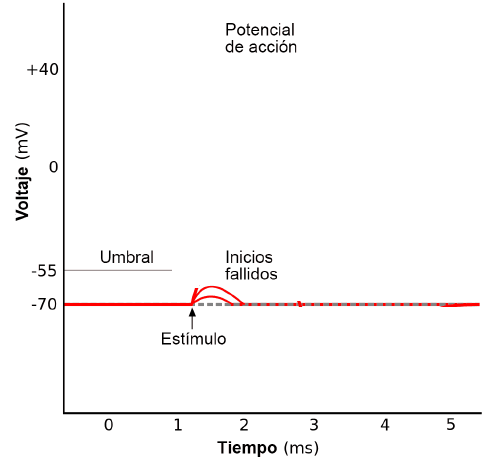
\includegraphics[scale=0.5]{Imagenes/Potencial_Accion_08b.png}
\end{figure}
\end{frame}
\begin{frame}
\frametitle{Despolarización}
En ese momento se genere la \textocolor{cobalt}{fase de despolarización} (canales de Na+ abiertos), \pause llegando al sobretiro que es la parte más elevada del potencial (canales de Na+ inactivos)
\end{frame}
\begin{frame}
\frametitle{Despolarización}
\begin{figure}
    \centering
    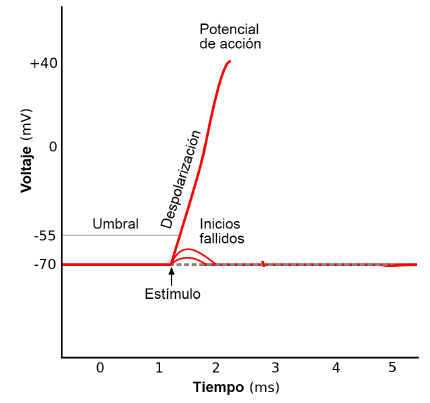
\includegraphics[scale=0.58]{Imagenes/Potencial_Accion_08c.png}
\end{figure}
\end{frame}
\begin{frame}
\frametitle{Repolarización}
Continuando la \textocolor{awesome}{repolarización} (canales de K+ abiertos), regresando al \textocolor{red}{estado de reposo}.
\end{frame}
\begin{frame}
\frametitle{Repolarización}
\begin{figure}
    \centering
    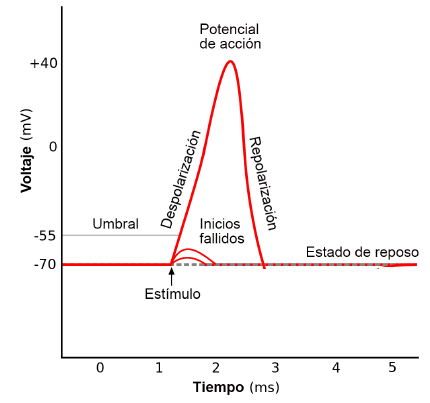
\includegraphics[scale=0.58]{Imagenes/Potencial_Accion_08d.png}
\end{figure}
\end{frame}
\begin{frame}
\frametitle{Periodo refractario}
El intervalo posterior al inicio de un potencial de acción en el que \textocolor{bole}{es imposible} o resulta más difícil producir una segunda espiga se denomina \textocolor{lava}{período refractario}.
\end{frame}
\begin{frame}
\frametitle{Periodo refractario}
\begin{figure}
    \centering
    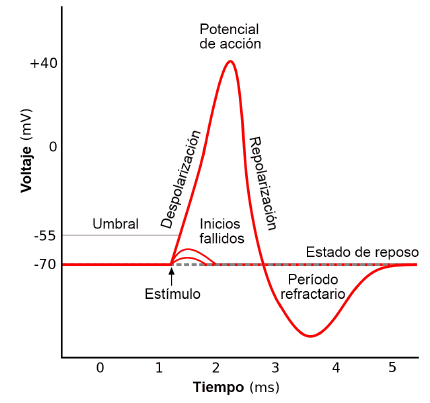
\includegraphics[scale=0.58]{Imagenes/Potencial_Accion_06.png}
\end{figure}
\end{frame}
\begin{frame}
\frametitle{Periodo refractario}
El periodo refractario consta de dos fases, el periodo refractario \textocolor{ao(english)}{absoluto} y el \textocolor{debianred}{relativo}.
\end{frame}
\begin{frame}
\frametitle{Periodo refractario absoluto}
El primero (absoluto) abarca desde el inicio del potencial de acción hasta casi el final de la repolarización.
\end{frame}
\begin{frame}
\frametitle{Periodo refractario absoluto}
En esta fase es imposible desencadenar un segundo potencial de acción, independientemente de la intensidad o duración del estímulo aplicado.
\end{frame}
\begin{frame}
\frametitle{Periodo refractario relativo}
El periodo \textocolor{cadmiumgreen}{refractario relativo} abarca el final de la repolarización y la hiperpolarización
\end{frame}
\begin{frame}
\frametitle{Hiperpolarización}
En la hiperpolarización, el estímulo necesario para que se lleve a cabo un nuevo potencial de acción deberá ser de mayor intensidad y duración que el estímulo que provocó el primer potencial de acción.
\end{frame}

\section{Resumen}
\frame{\tableofcontents[currentsection, hideothersubsections]}
\subsection{El potencial de acción}
% \section{El potencial de acción}
% \frame{\tableofcontents[currentsection, hideothersubsections]}
% \subsection{Definición}

\begin{frame}
\frametitle{¿Qué es el potencial de acción?}
El potencial de acción es un fenómeno eléctrico que ocurre en las \textocolor{ao}{células excitables}, como las neuronas y las células musculares.
\end{frame}
\begin{frame}
\frametitle{¿Qué es el potencial de acción?}
Es una \textocolor{red}{señal eléctrica rápida y temporal} \pause que se propaga a lo largo de la membrana celular.
\end{frame}
\begin{frame}
\frametitle{¿Qué es el potencial de acción?}
Tiene un papel fundamental en la comunicación celular y en la generación de respuestas específicas.
\end{frame}

\subsection{Características}

\begin{frame}
\frametitle{Umbral de excitación}
El potencial de acción se desencadena cuando el potencial eléctrico de la membrana alcanza un umbral crítico, llamado umbral de excitación.
\end{frame}
\begin{frame}
\frametitle{Umbral de excitación}
Este umbral debe superarse para que ocurra la despolarización de la membrana celular y se inicie el potencial de acción.
\end{frame}
\begin{frame}
\frametitle{Todo o Nada}
El potencial de acción sigue el principio de \enquote{\textocolor{red}{todo o nada}}
\end{frame}
\begin{frame}
\frametitle{Todo o Nada}
Lo que significa que una vez que se alcanza el umbral de excitación, \pause el potencial de acción se desencadena y tiene una amplitud y duración fija.
\end{frame}
\begin{frame}
\frametitle{Todo o Nada}
No importa la fuerza del estímulo que lo desencadene, siempre tendrá la misma amplitud y duración.
\end{frame}
\begin{frame}
\frametitle{Propagación}
Una vez iniciado, el potencial de acción \textocolor{debianred}{se propaga} a lo largo de la membrana celular en una dirección específica.
\end{frame}
\begin{frame}
\frametitle{Propagación}
Esto ocurre a través de un proceso llamado \textocolor{burntumber}{regeneración}.
\end{frame}
\begin{frame}
\frametitle{Potencial en propagación}
\begin{figure}
    \centering
    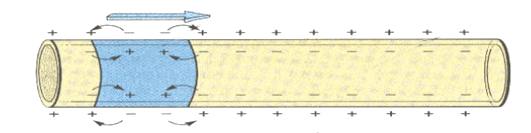
\includegraphics[scale=0.7]{Imagenes/Potencial_Accion_09a.png}
\end{figure}
\end{frame}
\begin{frame}
\frametitle{Potencial en propagación}
\begin{figure}
    \centering
    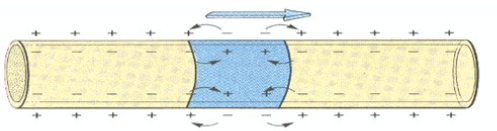
\includegraphics[scale=0.7]{Imagenes/Potencial_Accion_09b.png}
\end{figure}
\end{frame}
\begin{frame}
\frametitle{Potencial en propagación}
\begin{figure}
    \centering
    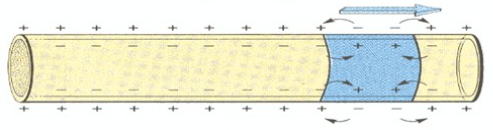
\includegraphics[scale=0.7]{Imagenes/Potencial_Accion_09c.png}
\end{figure}
\end{frame}
\begin{frame}
\frametitle{Regeneración}
En el cual la despolarización en un punto de la membrana activa canales iónicos vecinos, \pause desencadenando así el potencial de acción en esa región.
\end{frame}


\end{document}